\documentclass[10pt]{article}
\usepackage{amsmath,textcomp,amssymb,geometry,graphicx,enumerate,tikz,algorithm,algpseudocode,pifont,upgreek}
\usetikzlibrary{calc}
\usetikzlibrary{datavisualization}
\usetikzlibrary{datavisualization.formats.functions}


\textheight=9in
\textwidth=7in
\topmargin=-.75in
\oddsidemargin=-0.25in
\evensidemargin=-0.25in

\usepackage{listings}
\lstnewenvironment{codeblock}
    {\lstset{language=Python,
      showspaces=false,
      showtabs=false,
      breaklines=true,
      mathescape=true,
      showstringspaces=false,
      breakatwhitespace=true,
      commentstyle=\textit,
      keywordstyle=\textbf,
      basicstyle=\ttfamily,
      escapechar=`,
    }}
    {}

\newcommand{\bigo}{\mathcal{O}}
\newcommand{\R}{\mathbb{R}}


\begin{document}
\section*{04/11/2016}

\subsection*{Unsupervised Learning}
	\begin{itemize}
		\item We have sample points, but no labels!
		\item No classes, no y-values nothing to predict.
		\item Goal: Discover structure in the data.
		\item Example:
			\begin{itemize}
				\item Clustering: partition data into groups of similar/nearby points.
				\item Dimensionality reduction: data often lies near a low-dimensional subspace (or manifold) in feature space; matrices have low-rank approximations.
				\item Density estimation: fit a continues distribution do discrete data.
			\end{itemize}
	\end{itemize}
	
	\subsubsection*{Principal Component Analysis (PCA)}
	\begin{itemize}
		\item Goal: Given sample points in $\R^{d}$, find $k$ directions that capture the variation (dimensionality reduction).
			\begin{center}
				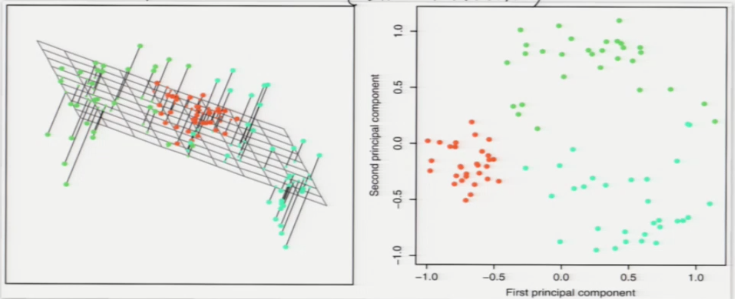
\includegraphics[scale=0.6]{../images/pca}
			\end{center}
		\item Why?
			\begin{itemize}
				\item Find a small basis for representing variations in complex things.
				\item Reducing number of dimensions make some computational cheaper, e.g. regression.
				\item Remove irrelevant dimensions to reduce overfitting in learning algorithms. Like subset selection, but we can choose features that aren't axis-aligned.
				\item 
			\end{itemize}
		\item Let $X$ be and $n$x$d$ design matrix.
		\item From now on assume $X$ is centered: mean $X_{i}$ is zero.
		\item Let $w$ be a unit vector.
		\item The \underline{orthogonal projection} of point $x$ onto vector $w$ is $\tilde{X}=(X \cdot w)w$.
		\item If $w$ not unit, $\tilde{x} = \frac{x \cdot w}{||w||^{2}} w$.
		\item Given orthonormal directions $v_{1}, \dots, v_{k}$ $\tilde{x} = \sum_{i=1}^{k} (x \cdot v_{i})v_{i}$. $x \cdot v_{i}$ are the coordinates in principal components space.
		\item $X^{T}X$ is square, symmetric, positive semidefinite, $d$x$d$ matrix.
		\item Let $0 \leq \lambda_{1} \leq \lambda_{2} \leq \dots \leq \lambda_{d}$ be its eigenvalues.
		\item Let $v_{1}, v_{2}, \dots, v_{d}$ be corresponding orthogonal unit eigenvectors.
		\item PCA Alg:
			\begin{itemize}
				\item Center $X$.
				\item Optional: Normalize $X$. Units of measurement different?
					\begin{itemize}
						\item Yes: Normalize.
						\item No: Usually don't.
					\end{itemize}
					\begin{center}
						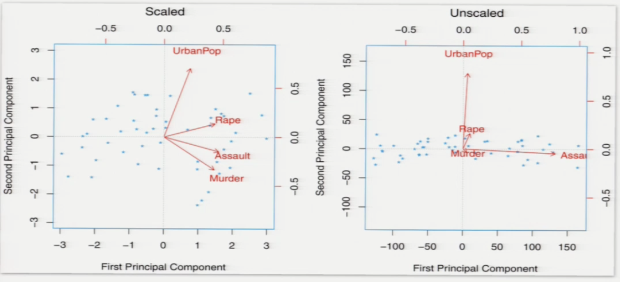
\includegraphics[scale=0.5]{../images/scaledcrime}
					\end{center}
				\item Compute unit eigenvectors/values of $X^{T}X$.
				\item Optional: choose $k$ based on the eigenvalue size.
					\begin{center}
						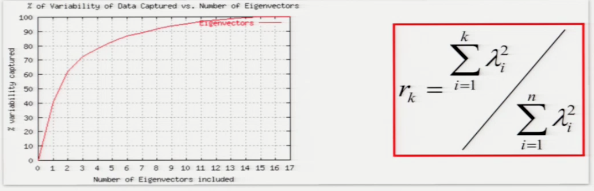
\includegraphics[scale=0.5]{../images/dimensionratio}
					\end{center}
				\item For the best $k$-dimensional subspace, pick directions $v_{d-k+1}, \dots, v_{d}$.
				\item Compute the coordinates of training/test data in principal components space.
			\end{itemize}
		\item PCA Derivations:
			\begin{enumerate}
				\item Fit a Gaussian to data with maximum likelihood estimation. Choose $k$ Gaussian axes of greatest variance. 
				\begin{center}
					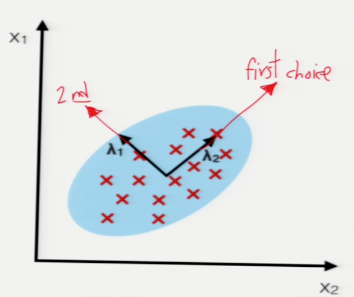
\includegraphics[scale=0.5]{../images/2dpca}
				\end{center}
				Recall that MLE estimates a covariance matrix $\hat{\Sigma} = \frac{1}{n} X^{T}X$
				
				\item Find direction $w$ that maximizes variance of projected data.
					\begin{align*}
						\text{Var}(\{\tilde{x_{1}}, \tilde{x_{2}}, \dots, \tilde{x_{n}}\}) &= \frac{1}{n} \sum_{i=1}^{n} \Big(X_{i} \cdot \frac{w}{|w|}\Big)^{2}\\
						&= \frac{1}{n} \frac{|Xw|^{2}}{|w|^{2}}\\
						&= \frac{1}{n} \frac{w^{T}X^{T}Xw}{w^{T}w}\\
					\end{align*}
					If $w$ is an eigenvector $v_{i}$, Rayleigh quotient = $\lambda_{i} \rightarrow$ of all eigenvector, $v_{d}$ achieves maximum variance $\frac{\lambda_{d}}{n}$. One can show $v_{d}$ beats every other vector too.
					Then pick $v_{d-1}$, then $v_{d-2}, \dots$
				
				\item Find direction $w$ that minimizes "projection error."
					\begin{align*}
						\sum_{i=1}^{n} |X_{i} - \tilde{X_{i}}|^{2} &= \sum |X_{i} - \frac{x_{i} \cdot w}{|w|^{2}}|^{2} = \sum (|X_{i}|^{2} - (X_{i} \cdot \frac{w}{|w|})^{2})\\
						&= \text{constant} - n\text{(variance from derivation 2)}.
					\end{align*}
					Minimizing projection error $\Leftrightarrow$ maximizing variance.
			\end{enumerate}
	\end{itemize}

\subsubsection*{Eigenfaces}
\begin{itemize}
	\item $X$ contains $n$ images of faces, $d$ pixels each.
	\item Face recognition: Given a query face, compare it to all training faces; find nearest neighbor in $\R^{d}$.
	\item Problem: Each query takes $\Theta(nd)$ time.
	\item Solution: Run PCA on faces. Reduce to much smaller dimension $d'$. Now nearest neighbor takes $\bigo(nd')$ time.
\end{itemize}

\end{document}